\section{AI in Software Testing}
% To achieve automatic test (data) generation from source code, there exists a well established framework: constraint-based testing~\cite{constraint,inka,dart,cute,onthefly}  (CBT). CBT approach focuses on translating part of a program into a logical formula whose solutions are relevant to test data. CBT also can be global, translating the whole program in a formula \cite{constraint,inka}, or local (path-based) \cite{dart,cute,onthefly}, focusing on a single path. In this report, we focus on path-based CBT, referred as path-based testing. 
% 
Symbolic execution~\cite{symbolic} is a way to track programs symbolicly rather than executing them with actual input value. Concolic path-based testing tools have literally blossomed up recently \cite{extenjpf,structural,mixed,exe,fuzz,pex} with the impressive progress in constraint solvers. Concolic path-based testing tools combine both concrete and symbolic execution (referred as concolic execution~\cite{dart,cute} or mixed execution~\cite{mixed}), which makes it possible to perform automatic path-based testing on large scale programs. By executing the program under test with concrete values while performing symbolic execution, symbolic constraints on the inputs can be collected from the predicates in branch statements, forming an expression, called path condition. To explore new paths, part of the constraints in the collected path conditions are negated to obtain new path conditions, which are sent to a constraint solver to compute test inputs for new paths. In theory, all feasible execution paths will be exercised eventually through the iterations of constraint collection and constraint solving in DSE.
% 
% A program under test can be modelled as a control flow graph (CFG)~\cite{testbook}, whose nodes represent simple primitive statements (such as input, output, and assignment) and edges represent the flow of control. An execution path of the program is a path on CFG from the starting node, entry of the program, to the exit node, exit of the program. Thus, to explore all paths of the program under test, i.e. achieving 100\% path coverage, is to enumerate all paths between two nodes in a graph, which is well known as a NP-hard problem~\cite{graph}. To alleviate this path explosion problem and to reduce the computation complexity, different AI techniques has been proposed, such as pruning search space of symbolic execution using heuristics~\cite{prune}, selective symbolic execution~\cite{selective} and fitness-guided path exploration~\cite{fitness}. In this report, we provide the details on pruning search space of symbolic execution using heuristics.

Recent and impressive progress in constraint solvers as well as the combination of both concrete and symbolic execution (referred as concolic execution~\cite{cute,dart}) make it possible to perform automatic path-based testing on large scale programs. However, these technologies are still suffering from two major bottlenecks: efficient constraint solving and the path explosion phenomenon. S\'{e}bastien Bardin and Philippe Herrmann~\cite{prune} focus on the second issue and propose three complementary heuristics geared toward lowering path explosion. All these heuristics deal with different distinct sources of path explosion. 

To cover all paths of a program is not the primarily objective of current testing practices. Often the case, it is only required to fully cover a class of structural artifacts of the program code source, such as statements, branches or atomic predicates. In the rest of the section, we denote these three classes of artifacts as structural coverage. There is an obvious mismatch between path-based approaches and such item coverage goals: while each new test data does cover a new path, it may hit no new item. Thus, path-based testing methods tend to waste a lot of time trying to compute irrelevant test data, i.e. test data exercising no new structural coverage. 

To address the path explosion issue in path-based testing with item coverage objectives, they provide three heuristics to discard irrelevant paths as much as possible, reducing of the number of solver calls and the whole computation time. The three heuristics are used as enhancements of a (bounded) depth-first search (DFS) path-based procedure, either purely symbolic or concolic. Original path-based testing techniques were based on DFS~\cite{dart,cute, onthefly}, while some recent works advocate using other search strategies~\cite{exe,hybrid,fuzz}.

\subsection{Look-Ahead heuristic}
\begin{figure}
\centering
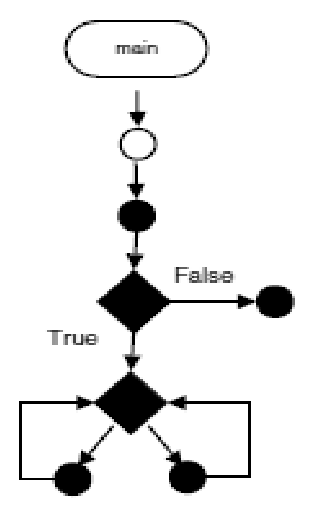
\includegraphics[scale=0.35,clip]{fig/la.eps} 
\caption{\label{fig:la}Example of Look-Ahead (LA) Heuristic} 
\end{figure}

The key idea of the Look-Ahead (LA) heuristic is to perform a reachability analysis in terms of reachable items in the CFG, and decide whether the current
path must be expanded based on the reachability analysis. If no new items can be reached, then exploration along the current path is stopped.

Figure \ref{fig:la} shows an example for illustrating the Look-Ahead (LA) heuristic. Let us assume the depth bound $k \geq 4$ and the objective is to achieve full statement coverage, and every path of the program is feasible. Then the original DFS based produre needs to explore $\approx2^k$ paths to achieve full coverage (because of the two nested loops) while DFS+LA requires at most 3 paths: one path to cover the false branch and two paths to cover two loops.

\subsection{Max-CallDepth (MCD) heuristic}
The major source of path explosion is function calls, and especially nested function calls. It is more embarrassing when only the top-level function is of interest. For example, the procedure may explore alternative (long) paths due to backtrack in deep callees while a simple backtrack at top-level would be sufficient. Example 1 of figure \ref{fig:mcd} gives such a behavior. Figure \ref{fig:mcd2} shows a small program where DFS achieves full branch coverage of main function with $k \geq 8$. DFS+MCD with mcd = 0 and any value of $k$ cannot cover one of the two branches of the main function, since a backtrack in sub-function $f$ is necessary. Consider the program of Figure \ref{fig:mcd}, take mcd = 0 and let us assume that sub-function f does not affect variable b. Then both DFS+LA+UT and DFS+MCD achieve full branch coverage. However, DFS+MCD explores only the two paths of function main, while DFS+LA explores $\approx 2^k$ paths. DFS+LA+MCD performs better
than DFS+LA in the example of Figure \ref{fig:mcd}, and it outperforms DFS+MCD in the example of Figure \ref{fig:la}.

\begin{figure}
\centering
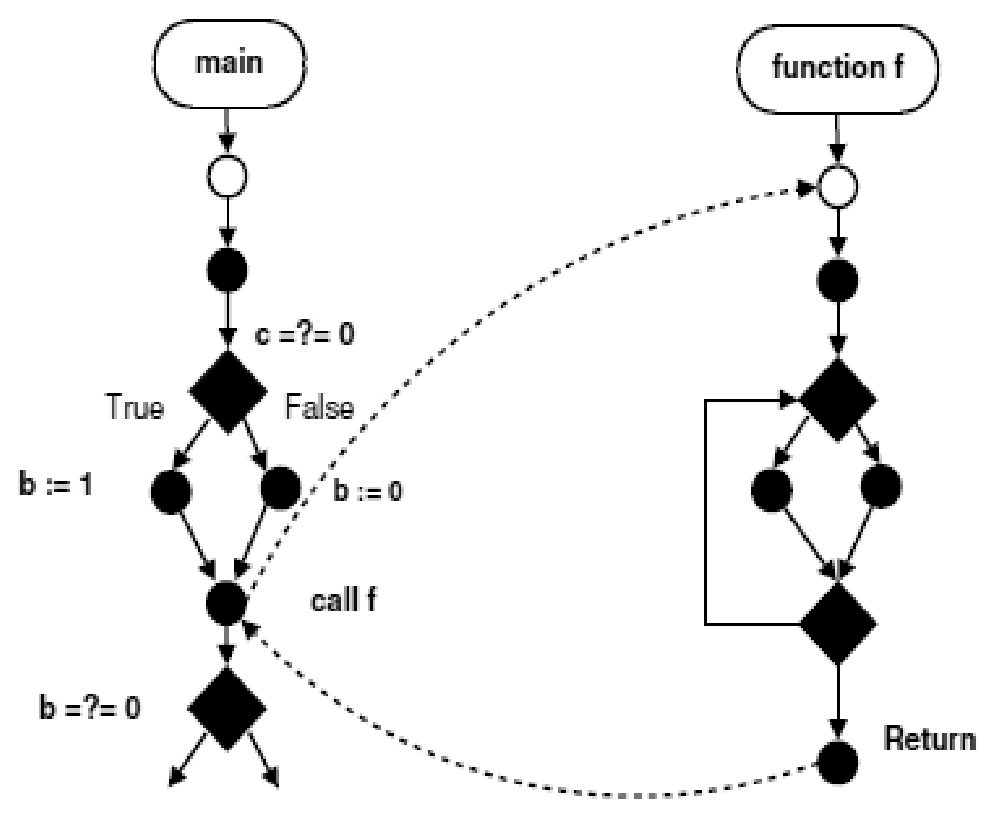
\includegraphics[scale=0.35,clip]{fig/mcd.eps} 
\caption{\label{fig:mcd}Example 1 of Max-CallDepth (MCD) heuristic} 
\end{figure}

The principle of the Max-CallDepth heuristic (MCD) is to prevent backtracking in deep nested calls, hoping such a deep decision is not mandatory to cover the function under test. It is clear that this heuristic makes sense only in unit testing. Moreover, contrary to LA, MCD may discard relevant paths and prevent the full coverage of the function under test. 

\begin{figure}[b]
\centering
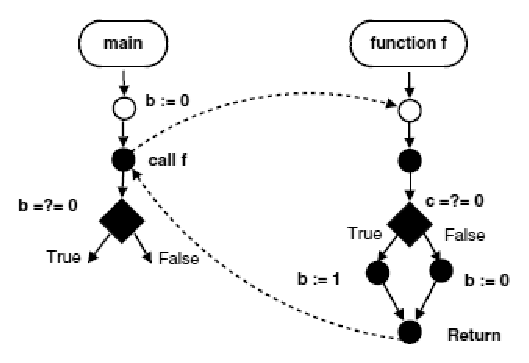
\includegraphics[scale=0.6,clip]{fig/mcd2.eps} 
\caption{\label{fig:mcd2}Example 2 of Max-CallDepth (MCD) heuristic} 
\end{figure}

\subsection{Solve-First (SF) heuristic}
Compared to other graph searches, DFS path exploration lowers memory consumption, since only one path at a time has to be maintained. However, DFS has at least two disadvantages in path-based testing. First, in a realistic environment where the number of tests we can run is limited, DFS may focus only on a very deep and narrow portion of the program under test and achieve only a poor global coverage. Second, DFS-based procedures explore and try to solve first the longest path prefixes, while shorter prefixes with probably simpler constraints may have covered the same items. Hence, DFS suffers from a slow initial coverage-speed and may waste resources on unduly complex paths.

\begin{figure}
\centering
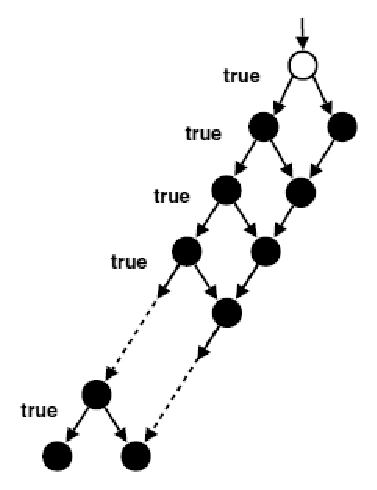
\includegraphics[scale=0.6,clip]{fig/sf.eps} 
\caption{\label{fig:sf}Example of Solve-First (SF) heuristic} 
\end{figure}

Solve-First heuristic (SF) is to partially address both issues described above, while keeping most of the advantages of DFS. SF is a DFS with the slight following modifications. When the procedure reaches a branch (choice point) for the first time, the first successor node is chosen as usual but all alternative successors are immediately resolved. Test data are derived from the solutions and executed in concrete mode to update coverage information. All solutions found are stored in a cache. On backtrack, once the next successor is chosen, the corresponding test
data is retrieved from the cache. The test data is then relaunched and the procedure proceeds as usual in the concolic case.

The program shown in Figure \ref{fig:sf} is parametrized by its number of nodes 2n + 1. Let us assume that all paths are feasible and that the first concrete path goes through every true branch. DFS+LA needs to explore n + 1 paths to achieve full instruction coverage while DFS+LA+SF
needs only to explore 2 paths. The depth bound for the concrete execution may be much larger than the one for concolic execution, allowing to cover more items. Note that essentially SF is concolic and has no interest in a symbolic setting.

\subsection{Conclusion and Related Work}
These three heuristics address the path explosion issue in common cases of irrelevancy. All these heuristics are lightweight, both in terms of implementation cost and computational overhead, and they are all complementary since each one addresses a typical source of path explosion.
Their evaluations show that these heuristics have a significant impact on the number of paths considered and overall performances. Although these three techniques have been presented in a DFS framework, they are easy to adapt to other path-based frameworks. 

